\documentclass[12pt,oneside,titlepage,openright,a4paper]{book}
\usepackage[utf8]{inputenc}
\usepackage[style=numeric,sorting=none]{biblatex}
\bibliography{Tesis}
\usepackage[hidelinks]{hyperref}
\usepackage[version=3]{mhchem} % Formula subscripts using \ce{}
\usepackage{pdflscape}
%\usepackage{ucs}
%\usepackage{uarial}
\usepackage[spanish,english]{babel}
\usepackage{csquotes}
\usepackage{latexsym}
\usepackage{amssymb,amsmath,amsthm,amsfonts}
\usepackage{fancyhdr}
\usepackage{fancybox}    
\usepackage{t1enc}
\usepackage{array}
\usepackage[pdftex]{graphicx}
\usepackage[below]{placeins}
\usepackage{float}
\usepackage{caption}
\usepackage{rotating,colortbl,longtable,tabulary,booktabs}
\usepackage{tocbibind}
\usepackage{wrapfig,subfigure}
\usepackage{tikz,pgfkeys,tkz-base}
\usepackage{comment} % enables the use of multi-line comments (\ifx \fi)
\usepackage{fullpage} % changes the margin
\usepackage{multirow, array}
\usepackage[left=3cm,right=2.5cm,top=2cm,bottom=2cm]{geometry}
\usepackage{appendix}
\usepackage{lmodern}
\usepackage{booktabs}
\usepackage{lscape}
\usepackage{pdflscape}
\usepackage{rotating}
\usepackage{url}
\usepackage{color}
\definecolor{Mygray}{gray}{0.85}
\usepackage{xcolor}
% \newcounter{subsubsubsection} [subsubsection]
\setcounter{secnumdepth}{3}
\usetikzlibrary{arrows,decorations.pathmorphing,backgrounds,positioning,fit,trees,calc,through,plotmarks}
%\bibpunct{}{,}{} 
\setlength{\parindent}{0.5cm}
\setlength{\parskip}{0.2cm}
\linespread{1.5}
\usepackage{eso-pic}
\newcommand\BackgroundPic{
\put(0,0){
\parbox[b][\paperheight]{\paperwidth}{%
\vfill
\centering
\includegraphics[width=0.75\paperwidth,height=\paperheight,keepaspectratio]{figuras/ib.png}%
\vfill
}}}
%--------------------------------------------------------------------------------------------------------------------------------------------------------------------
\begin{document}
\AddToShipoutPicture{\BackgroundPic}
\renewcommand{\tablename}{Tabla}
\renewcommand{\listtablename}{Índice de Tablas}
\renewcommand{\contentsname}{Contenido}
\renewcommand{\listfigurename}{Índice de Figuras}
\renewcommand{\chaptername}{Capítulo}
\begin{titlepage}
\begin{center}
\textbf{\begin{LARGE}Universidad Católica de Santa María \end{LARGE}}\\
\begin{Large}Facultad de Ciencias Farmacéuticas, Bioquímicas y Biotecnológicas\end{Large}\\
\begin{large}Escuela profesional de Ingeniería Biotecnológica\end{large}\\\vspace{2.0cm}
\includegraphics[scale=0.2]{figuras/logo.png}\\\vspace{2.0cm}
\textbf{\begin{LARGE} Interacción de metabolitos secundarios del Aloe Vera como inhibidores potenciales de la dipeptidil peptidasa-4 (DPP4) postulándolos como alternativas a tratamiento de Diabetes Mellitus tipo 2 (DMT2)
\end{LARGE}}\\\vspace{2.0cm}
\end{center}
\begin{flushright}
\begin{minipage}{7cm}
Tesis presentada por el Bachiller:\\ \textbf{Quispe Ppacco, David Jonatán}\\ 
Para Optar el Titulo Profesional de:\\  \textbf {Ingeniero Biotecnólogo} \\
Asesor:\\ Gómez Valdez, Badhin
\end{minipage}
\end{flushright}
\vspace{0.5cm}
\begin{center}
\begin{Large}\textbf{Arequipa -- Perú\\2024}\end{Large}
\end{center}
\end{titlepage}
%--------------------------------------------------------------------------------------------------------------------------------------------------------------------
\pagenumbering{arabic}\tableofcontents 
%--------------------------------------------------------------------------------------------------------------------------------------------------------------------
\chapter{Introducción}
La Diabetes se encuentra entre las diez enfermedades con alta mortalidad en adultos, presentando una prevalencia del 9,3\% en el año 2019 y según predicciones se puede esperar un aumento del 0,9\% para el año 2030. %Rachin%

Las investigaciones nos indican que existen otros blancos disponibles como lo es el tratamiento de la DMT2 aumentando la prevalencia de la activación de la via de señalización dependiente de GLP1, evitando su inhibición por la enzima Dipeptidil peptidaza 4 (DPP4) mencionada proteína puede inhibirse por diversos fármacos del grupo de las gliptinas, como lo es la Vildagliptina entre otras. %Buscaridea%

El objetivo de mencionadas investigaciones fueron el de encontrar diversos compuestos que puedan reducir la intervención farmacéutica o solo reducirla para poder ser reemplazada por algún metabolito proveniente de agentes naturales como lo son las plantas. %buscar idea%

En esta investigación nos centraremos en el potencial de diversos metabolitos encontrados en el aloe vera para poder ser comparados y encontrar diferencias significativas entre el uso de los agentes farmacológicos y los agentes naturales. viendo las diferencias podremos afirmar si los agentes derivados del aloe vera podrían ser similares, o mejores que los agentes farmacológicos. %buscar idea% 
\chapter{Planteamiento de la Investigación}
\renewcommand{\figurename}{Figura}
La Diabetes se encuentra entre las diez enfermedades con alta mortalidad en adultos, presentando una prevalencia del 9,3\% en el año 2019 y según predicciones se puede esperar un aumento del 0,9\% para el año 2030. %Rachin%
Esta alarma no es indiferente a la búsqueda de soluciones alternativas para tratar mencionada enfermedad, existen diversos métodos y tratamientos que se han expuesto a la sociedad como son medicamentos asociados a reducir la glucosa en la sangre como los son la metformina que es uno de más usados actualmente.%Buscar idea%
Las investigaciones nos indican que existen otros blancos disponibles como lo es el tratamiento de la DMT2 aumentando la prevalencia de la activación de la via de señalización dependiente de GLP1, evitando su inhibición por la enzima Dipeptidil peptidaza 4 (DPP4) mencionada proteína puede inhibirse por diversos fármacos del grupo de las gliptinas, como lo es la Vildagliptina entre otras. %Buscaridea%

Se ha querido encontrar diversos metabolitos que puedan evitar la interacción farmacéutica o solo reducirla para poder ser reemplazada por algún metabolito proveniente de agentes naturales como lo son las plantas. %buscar idea%
En esta investigación nos centraremos en el potencial de diversos metabolitos encontrados en el aloe vera para poder ser comparados y encontrar diferencias significativas entre el uso de los agentes farmacológicos y los agentes naturales. viendo las diferencias podremos afirmar si los agentes derivados del aloe vera podrían ser similares, o mejores que los agentes farmacológicos. %buscar idea% 

\section{Problemática de la investigación}

Según lo encontrado por Rachi et al podemos afirmar que la prevalencia de Diabetes irá en aumento hasta llegar a un nivel de aumento del 0,9-1\% de prevalencia en aproximadamente 5 años, es por ello que se requiere de nuevas tecnologías que puedan ayudar al tratamiento o control de mencionada patología.
Dentro de la problemática principal como lo es el aumento de la prevalencia de los casos de diabetes a nivel global, esto trae consigo problemas asociados como lo son las neuropatías, daño renal, retinopatías entre otras.%Publications%
Por otro lado se ha observado que la Metformina ha empezado a presentar algunos efectos secundarios en gente adulta como lo son malestares gástricos e intestinales los cuales han forzado a los tratamientos ayudarse del grupo de los fármacos como las gliptinas para poder ayudar a estos cambios siendo la solución la inhibición de la proteína DPP4.

Finalmente el consumo de fármacos seguirá en crecimiento durante este aumento de la prevalencia de Diabetes es por ello que es mejor optar por otras opciones aparte de los fármacos y tratamientos convencionales enfocándonos en la naturaleza, es por ello que haciendo un análisis de posibles inhibidores postulamos al aloe vera como uno de los posibles portadores de metabolitos secundarios que puedan contener compuestos que interaccionen a nivel del intestino y estómago con fundamento a los antecedentes que presenta mencionada planta frente a la diabetes.

\section{Pregunta de investigación}
Dentro del análisis de datos obtenidos de los antecedentes del aloe vera con la diabetes ¿Es posible mencionar que los metabolitos secundarios encontrados en el aloe vera presenten mayor capacidad inhibitoria que los  fármacos convencionales que interactúan con la proteína DPP4 para el control de la Diabetes Mellitus tipo 2 (DMT2)?

\section{Justificación}


\section{Alcance}


\section{Objetivos}

\subsection{General}


\subsection{Específicos}

\begin{itemize}
 \item 
\item 
\item 

\end{itemize}

\section{Hipótesis}



\section{Variables e indicadores}

 \begin{table}[htbp]
 \caption{Cuadro de variables}\label{t1}
\begin{tabular}{lllccc}
\hline
\multicolumn{3}{c}{\textbf{Variables}}                       & \textbf{Variable}      & \textbf{Indicadores}                 & \textbf{Unidades} \\ \hline
\multicolumn{3}{c}{\multirow{2}{*}{\textbf{Independientes}}} &   &   & \\ \cline{4-6} 
\multicolumn{3}{c}{}                                         &   &   & \\ \hline
\multicolumn{3}{l}{\multirow{4}{*}{\textbf{Dependientes}}}   &   &   & \\ \cline{4-6} 
\multicolumn{3}{l}{}                                         &   &   & \\ \cline{4-6} 
\multicolumn{3}{l}{}                                         &   &   & \\ \cline{4-6} 
\multicolumn{3}{l}{}                                         &   &   & \\ \hline
\end{tabular}
\end{table}

\section{Tipo y Nivel de Investigación}




\chapter{Antecedentes}
\renewcommand{\figurename}{Figura}

\section{Estado del Arte}
En el artículo titulado "Phthalate-induced testosterone/androgen receptor pathway disorder on spermatogenesis and antagonism of lycopene" publicado en el año de 2022, se detalla que la vía de señalización de testosterona (T)/receptor de andrógenos (AR) está involucrada en el mantenimiento de la espermatogénesis y la fertilidad masculina. Los resultados obtenidos en la investigación demostraron que el ftalato de mono-2-etilhexilo (MEHP) causó daño mitocondrial y daño oxidativo, por lo que se determinó que esta sustancia química seria amenaza para el progreso de la espermatogénesis. Sin embargo, en la investigación también realizaron estudios antagonistas del licopeno frente a la alteración que produce los ftalatos en el trastorno de la vía del receptor de andrógenos/ testosterona, teniendo como resultados que este suplemento LYC es una agente antioxidante natural que inhibe los cambios producidos por los ftalatos frente la función espermatogénica de los testículos. En general, este estudio revelo un papel fundamental para la transducción de señales T/AR en la fertilidad masculina y proporciono información prometedora sobre el papel protector de LYC en los trastornos reproductivos masculinos inducidos por ftalatos.\cite{b12}



\chapter{Marco Teórico}

 \section {Título de la sección}
 
 
\subsection{Título de la subsección}



 
\chapter{Planteamiento Metodológico}

Para la metodología se optó por el campo computacional usando softwares especializados en lo que es interacciones y dinámicas moleculares

\section{Lugar en donde se desarrollará la investigación}
El lugar donde se desarrollará esta investigación es en Centro de Investigación en Ingeniería Molecular (CIIM) autorizado y supervisado por el Dr. Badhin Gómez Valdez   

\section{Ambientes por utilizar}
Se usaran los ambientes asociados al centro de investigación cuya estación de trabajo está preparada y optimizada para generar los resultados esperados dentro de la preparación, dinámica y análisis molecular. 

\section{Materiales}
Para esta investigación se han de requerir computadores óptimos para los cálculos cuánticos que se tienen que llevar a cabo:

\subsection{Hardware}
\begin{itemize}
    \item Procesador AMD Ryzen 9 
    \item Placa madre X570 gaming
    \item GPUs NVIDIA 3080 y NVIDIA 2080
    \item sistemas de ventilación optimizados
    \item Fuente de poder de Seasonic 80 Plus Gold
\end{itemize}

\subsection{Software}
\begin{itemize}
    \item Sistema operativo Linux 24.04
    \item Chimera X
    \item AlphaFold3 (Nativo)
    \item Autodock Vina (Nativo)
    \item Gromacs v.2024.3 
    \item Gaussian y derivados
\end{itemize}

\section{Métodos}

\subsection{Interacción proteica en estado basal de la enzima DPP4}
Para ello haremos uso de los softwares de predicción de modelos proteicos como lo es el modeller integrado en el software Chimera X al igual que AlphaFold3 que tienen la finalidad de predecir el estado de la proteína por comparación.

El primero objetivo a cumplir es la extracción de la proteína de una base de datos como lo es Protein Data Bank (PDB) luego de encontrar la enzima adecuada verificando la mejor valoración según bibliografía procedemos a realizar la construcción de la molécula si lo necesita, posterior a ello procedemos a la búsqueda de la proteína blanco como lo es el Péptido Parecido al Glucagón (GLP1) de la misma forma valoramos por búsqueda bibliográfica los estadios de la molécula y usamos softwares de modelado si esto lo requiere, Softwares como AlphaFold que mejora considerablemente al tenerlo integrado a la máquina donde se trabajará el modelado de las proteínas.

Después de haber realizado la limpieza de las proteínas y completado todos los residuos a utilizar si estos lo requieren. Generamos dinámicas moleculares usando GROMACS como software y OPLS como campo de fuerza a las proteínas por separado, esto con el fin de estabilizar ambas proteínas y encontrar su estado basal independiente gracias a los gráficos de dinámica.
Posterior a ello procederemos a la interacción proteica esto se realizará con un dockeo a nivel citoplasmático como es normalmente, en este caso mantenemos la GLP1 estable mientras que la enzima dse aproxima como ligando, normalmente mientras más veces repita el Autodock vina presenta mejor probabilidad estadística de brindar un resultado estable donde podemos afirmar el valor inhibitorio en estado basal de ambas moléculas cuando interaccionan en el estado de catálisis enzimática.

\subsection{Generación de la base de datos de ligandos}
Para este punto se requiere del análisis de bibliografía especializada en ligandos de interés como pueden ser ligandos encontrados en el Aloe Vera con aplicaciones antidiabéticas pero también los ligandos encontrados para otras funciones podrían ser resultados favorables es por ello que hacemos una búsqueda de aproximadamente 113 metabolitos gracias a diferentes bases de datos los cuales serán filtrados por bibliografía y por el estándar ADMET que nos ayudará a buscar los mejores resultados para tener valores altos de druagabilidad protética y así generar la inhibición de DPP4.

Finalmente usaremos la base de datos de estudios previos farmacológicos que nos agreguen la mayor cantidad de fármacos comerciales sintetizados con la finalidad de generar la inhibición de DPP4. Estos fármacos presentan a la familia de las gliptinas como una de las más importantes pero se agregarán muchos mas dependiendo del análisis bibliográfico y el filtro ADMET que nos ayudará a buscar estadísticamente los mejores resultados para la interacción como ligandos inhibidores de la actividad enzimática de la DPP4. 

\subsection{Análisis de resultados por dinámica molecular y análisis estadístico}
Dependiendo de los resultados generaremos un análisis de los mejores ligandos tanto de los ligandos sintéticos como de los de procedencia natural ya que la liste ha reducido considerablemente se pude realizar un ultimo dockeo con el fin de encontrar diferencias en las energías de interacción ya que de esta evaluación se generará un análisis estadístico para evidenciar los mejores ligandos con mejor potencial inhibitorio decidiendo finalmente si los metabolitos extraídos del aloe vera podrían superar la inhibición de los actuales fármacos usados para el tratamiento de la Diabetes Mellitus Tipo 2.

\section{Flujograma de actividades }

%\begin{figure}
 %   \centering
 %   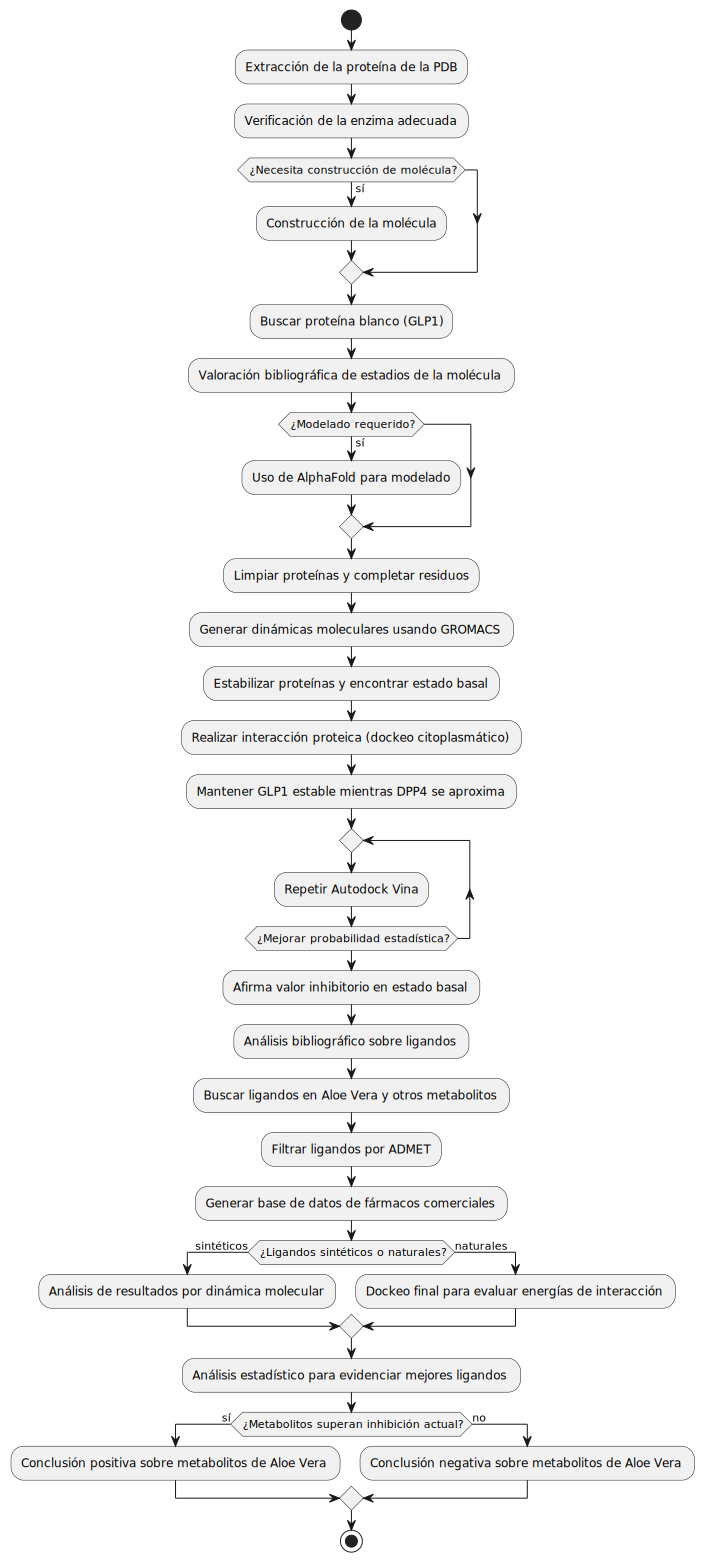
\includegraphics{figuras/Flujograma.svg}
 %   \caption{Figura}
 %   \label{Flujograma}
%\end{figure}




\chapter{Cronograma y Presupuesto de la Investigación}

\newpage
\section{Cronograma} 
\begin{table}[!htb]
\begin{center}
\begin{tabular}{|p{7cm}|c|c|c|c|c|c|c|c|c|c|c|c|}\hline
\multirow{2}{*}{\textbf{Actividades}}    & \multicolumn {12}{c|}{\textbf{Meses}} \\\cline{2-13}
                                              & 1 & 2 & 3 & 4 & 5 & 6 & 7 & 8 & 9 & 10 & 11 & 12\\\hline
                                              &   &   &   &   &   &   &   &   &   &    &    &   \\\hline
                                              &   &   &   &   &   &   &   &   &   &    &    &   \\\hline    
                                              &   &   &   &   &   &   &   &   &   &    &    &   \\\hline
                                              &   &   &   &   &   &   &   &   &   &    &    &   \\\hline  
                                              &   &   &   &   &   &   &   &   &   &    &    &   \\\hline
                                              &   &   &   &   &   &   &   &   &   &    &    &   \\\hline  
                                              &   &   &   &   &   &   &   &   &   &    &    &   \\\hline
                                              &   &   &   &   &   &   &   &   &   &    &    &   \\\hline  
                                              &   &   &   &   &   &   &   &   &   &    &    &   \\\hline
                                              &   &   &   &   &   &   &   &   &   &    &    &   \\\hline  
                                              &   &   &   &   &   &   &   &   &   &    &    &   \\\hline
                                              &   &   &   &   &   &   &   &   &   &    &    &   \\\hline                                                
\end{tabular} 
\end{center}
\end{table}


\newpage
\section{Presupuesto}

Financiado por el fondo 
 
%\include{referencias}
%--------------------------------------------------------------- ---------------------------------------------------------------------------------------------------------------------------------------------------
%\bibliographystyle{vancouver}
%\renewcommand{\bibname}{Referencias Bibliográficas}
%\bibliography{Tesis} 
%\appendix
%\addcontentsline{toc}{chapter}{Anexos}
\part*{Anexos}

\printbibliography

%--------------------------------------------------------------------------------------------------------------------------------------------------------------------
\end{document}
%-------------------------------------------------------------------------------------------------------------------------------------------------------------------- 
